\documentclass[
10pt, % Set the default font size, options include: 8pt, 9pt, 10pt, 11pt, 12pt, 14pt, 17pt, 20pt
%t, % Uncomment to vertically align all slide content to the top of the slide, rather than the default centered
aspectratio=169, % Uncomment to set the aspect ratio to a 16:9 ratio which matches the aspect ratio of 1080p and 4K screens and projectors
]{beamer}

\usepackage[all]{xy}

\usepackage[spanish]{babel}
\usepackage[utf8]{inputenc}

\graphicspath{{Images/}{./}} % Specifies where to look for included images (trailing slash required)

\usepackage{booktabs} % Allows the use of \toprule, \midrule and \bottomrule for better rules in tables

%\usepackage{tikz}
%\usetikzlibrary{positioning}
%\usetikzlibrary{shapes,arrows,arrows,positioning,fit}

\usepackage{tikz}
\usepackage{adjustbox}
\usetikzlibrary{arrows, shapes}

\usepackage{forest}

\usepackage{multirow}

\usepackage{graphicx}
\usepackage{hyperref}

\usepackage{xcolor,listings}
\usepackage{textcomp}
%\usepackage{color}

\usepackage{enumitem}

\usepackage{xcolor}

\usepackage{verbatim}
\usepackage{changepage}

\usepackage{algorithm}
\usepackage{algpseudocode}
\usepackage{gensymb}

\usepackage{venndiagram}

\usepackage{graphicx}

\usepackage{array}

\usepackage{colortbl}
\usetikzlibrary{positioning}

\usepackage{pgfplots}

% \usepackage{media9}

% \usepackage{algorithm}
% \usepackage{algorithmic}

\providecommand{\abs}[1]{\lvert#1\rvert}

%----------------------------------------------------------------------------------------
%	SELECT LAYOUT THEME
%----------------------------------------------------------------------------------------
\usetheme{Madrid} 

%----------------------------------------------------------------------------------------
%	SELECT COLOR THEME
%----------------------------------------------------------------------------------------
%\usecolortheme{beaver}
%\usecolortheme{seahorse}
\usecolortheme{spruce} % verde suave
%\usecolortheme{whale}
%\usecolortheme{wolverine}

%----------------------------------------------------------------------------------------
%	SELECT FONT THEME & FONTS
%----------------------------------------------------------------------------------------
\usefonttheme{default} % Typeset using the default sans serif font
%\usefonttheme{serif} % Typeset using the default serif font (make sure a sans font isn't being set as the default font if you use this option!)
%\usefonttheme{structurebold} % Typeset important structure text (titles, headlines, footlines, sidebar, etc) in bold
%\usefonttheme{structureitalicserif} % Typeset important structure text (titles, headlines, footlines, sidebar, etc) in italic serif
%\usefonttheme{structuresmallcapsserif} % Typeset important structure text (titles, headlines, footlines, sidebar, etc) in small caps serif

%------------------------------------------------

%\usepackage{mathptmx} % Use the Times font for serif text
%\usepackage{palatino} % Use the Palatino font for serif text

\usepackage{helvet} % Use the Helvetica font for sans serif text
%\usepackage[default]{opensans} % Use the Open Sans font for sans serif text
%\usepackage[default]{FiraSans} % Use the Fira Sans font for sans serif text
\usepackage[default]{lato} % Use the Lato font for sans serif text

%----------------------------------------------------------------------------------------
%	SELECT INNER THEME
%----------------------------------------------------------------------------------------
\useinnertheme{circles}


\setbeamertemplate{footline} % Uncomment this line to remove the footer line in all slides
%\setbeamertemplate{footline}[page number] % Uncomment this line to replace the footer line in all slides with a simple slide count

\setbeamertemplate{navigation symbols}{} % Uncomment this line to remove the navigation symbols from the bottom of all slides

%----------------------------------------------------------------------------------------
%	PRESENTATION INFORMATION
%----------------------------------------------------------------------------------------

\title[Short Title]{Acercamiento a la minería en redes} 

\subtitle{Sistemas de Recuperación de Información}

\author{Lic. Carlos León González \\ Dra.C. Lucina García Hernández}

\institute[UC]{Facultad de Matem\'atica y Computaci\'on \\ Universidad de La Habana \\ \smallskip }

\date{18 de marzo de  2024} % Presentation date or conference/meeting name, the optional parameter can contain a shortened version to appear on the bottom of every slide, while the required parameter value is output to the title slide

%----------------------------------------------------------------------------------------

\begin{document}
	
	\lstset{
		literate=%
		{á}{{\'a}}1
		{í}{{\'i}}1
		{é}{{\'e}}1
		{ý}{{\'y}}1
		{ú}{{\'u}}1
		{ó}{{\'o}}1
		{ě}{{\v{e}}}1
		{š}{{\v{s}}}1
		{č}{{\v{c}}}1
		{ř}{{\v{r}}}1
		{ž}{{\v{z}}}1
		{ď}{{\v{d}}}1
		{ť}{{\v{t}}}1
		{ň}{{\v{n}}}1                
		{ů}{{\r{u}}}1
		{Á}{{\'A}}1
		{Í}{{\'I}}1
		{É}{{\'E}}1
		{Ý}{{\'Y}}1
		{Ú}{{\'U}}1
		{Ó}{{\'O}}1
		{Ě}{{\v{E}}}1
		{Š}{{\v{S}}}1
		{Č}{{\v{C}}}1
		{Ř}{{\v{R}}}1
		{Ž}{{\v{Z}}}1
		{Ď}{{\v{D}}}1
		{Ť}{{\v{T}}}1
		{Ň}{{\v{N}}}1                
		{Ů}{{\r{U}}}1    
	}
	
	
	\begin{frame}
		\titlepage
	\end{frame}
	
	%------------------------------------------------
	% Objetivos
	\begin{frame}
		
		\frametitle{Objetivos}
		
		\begin{itemize}

			\item Explorar las principales propiedades de las redes y sus diferentes topologías. \\[2mm]
			
			\item Explorar diferentes medidas de centralidad del nodo. \\[2mm]
			
			\item Comprender las ventajas y los problemas de la detección de comunidades .
			
		\end{itemize}
		
	\end{frame}
	
	%------------------------------------------------
	%  
	\begin{frame}
		
		\frametitle{¿Qué información a priori puede extraerse de un grafo?}
		
		\centering
		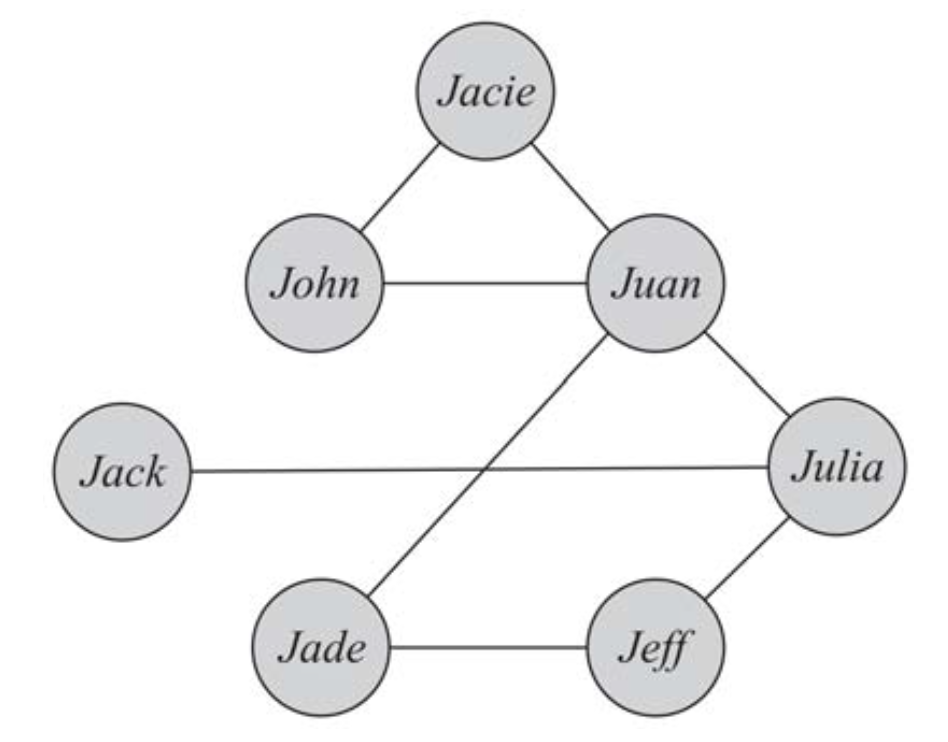
\includegraphics[scale=0.5]{g1.png}
		
		\only<2>{
			\textcolor{purple}{¿Qué algoritmos \textbf{existen} para extraer información de un grafo, según lo estudiando en años anteriores?}
		}
		% Componentes fuertemente conexas
		% Aristas de corte
		% Puntos de articulación
		
		% PageRank 
		% Algoritmos clásicos de grafos como: 
		% 	- componentes fuertemente conexas
		% 	- puntos de articulación y aristas de corte
		
	\end{frame}
	
	%------------------------------------------------
	%  Motivación
	\begin{frame}
		
		\frametitle{¿Por qué se ha prestado especial atención al análisis de las redes?}
		
		Analizar una red permite:
		\begin{itemize}
			
			\item Encontrar nodos ``sensibles'' \\[1mm]
			% Esto puede ser xq x ellos pasan todo el tráfico de la red, o porque están aislados y contienen datos importantes de otros nodos.
			
			\item Analizar la topología de la red \\[1mm]
			% Optimización de recursos
			% Seguridad  
			
			\item Detectar de anomalías y seguridad \\[1mm]
			% identificar patrones inusuales o comportamientos anómalos en la red que podrían indicar intrusiones o actividades maliciosas.
			
			\item Detectar tendencias antes de que se conviertan en tendencia \\[1mm]
			% Los datos disponibles en las plataformas de redes sociales pueden brindar información importante sobre la sociedad y el comportamiento de los usuarios. Las empresas pueden analizar las palabras clave, los resultados de búsqueda, los comentarios y las menciones para identificar la tendencia actual, y un estudio más profundo del cambio de comportamiento también puede ayudar a predecir tendencias futuras. Estos datos son muy útiles para que las empresas tomen decisiones informadas cuando hay mucho en juego.
			
			\item Detectar patrones 
			
			\item Establecer macro-relaciones 
			
		\end{itemize}
		
	\end{frame}
	
	%------------------------------------------------
	%  Ejemplos de grafos
	\begin{frame}
		
		\frametitle{Ejemplos de grafos en la vida real}
		
		\begin{itemize}
			\item Red social
			\item Red de transporte
			\item Grafo de Internet
			\item Mapa conceptual
			\item Red de computadoras
			\item Modelo de flujo
		\end{itemize}
		
		\vspace{2\baselineskip}
		Basta con tener un conjunto de entidades y relaciones entre ellas para modelar la problemática en una representación de grafo. 
				
	\end{frame}
	
	%------------------------------------------------
	%  Propiedades de las redes 
	\begin{frame}
		
		\frametitle{Propiedades de las redes}
		
	\begin{itemize}
		\item Las redes del mundo real comparten características y atributos comunes. \\[4mm]
		% Los análisis se apoyan de estas características, siendo una práctica común identificar sus atributos y mostrar que las mediciones de estos atributos son consistentes en todas las redes.
		
		\item Los atributos que exhiben mediciones consistentes son:
		\begin{itemize}

			\item Distribución del grado de los nodo
			% Denota cómo se distribuyen los grados de los nodos en una red.

			\item Coeficiente de agrupamiento
			% Mide la transitividad de una red.
			% La transitividad en una red se refiere a la probabilidad de que si un nodo A está conectado con un nodo B, y el nodo B está conectado con un nodo C, entonces existe una alta probabilidad de que el nodo A también esté conectado con el nodo C.

			\item Longitud promedio del camino
			% Denota la distancia promedio (longitud de ruta más corta) entre pares de nodos.

		\end{itemize}
		
	\end{itemize}
		
	\end{frame}
	
	%------------------------------------------------
	%  Propiedades de las redes: Distribución del grado de cada nodo
	\begin{frame}
		
		\frametitle{Propiedades de las redes: Distribución del grado de cada nodo}
		
		\begin{alertblock}{}
			El grado (\emph{degree}) de un nodo es la cantidad de aristas conectadas al nodo en un grafo no dirigido. Para el caso de grafos dirigidos se establece una diferencia entre la cantidad de aristas que entran al nodo (\emph{indegree}) y las aristas que salen (\emph{outdegree}), siendo \emph{degree $=$ indegree $+$ outdegree}.
		\end{alertblock}
		
		\vspace{1.5\baselineskip}
		
		Por ejemplo:
		\begin{itemize}
			\item Red social: El grado de un nodo representa la popularidad de la entidad o el nivel de interés de otras entidades hacia esta.
			\item Red de ingredientes de recetas de cocina: El grado de un nodo representa el nivel de importancia o de frecuencia de uso de ese ingrediente en la cocina. 
		\end{itemize}
		
	\end{frame}
	
	%------------------------------------------------
	%  Propiedades de las redes: Distribución del grado de cada nodo
	\begin{frame}
		
		\frametitle{Propiedades de las redes: Distribución del grado de cada nodo}
		
		\begin{minipage}{0.45\textwidth}
		
			La probabilidad de encontrar nodos de grado $k$ en el grafo es:
			$$p_k = \frac{n_k}{n} $$
			
			\only<1>{
				donde: 
				\begin{itemize}
					\item $V$ conjunto de nodos del grafo
					\item $n_k = |{v: v \in V, \text{degreee}(n) = k }|: $
					\item $n = |V|$
				\end{itemize}
			}
			
			\only<2>{
				\vspace{1\baselineskip}
				
				% La distribución de ley de potencia, también conocida como distribución de cola pesada, es un tipo de distribución de probabilidad en la que las probabilidades de los eventos de alta magnitud siguen una ley de potencia. Esto significa que la probabilidad de que un evento ocurra con una magnitud muy grande es mucho mayor que bajo una distribución normal o exponencial.
				
				Existe el mismo comportamiento que la Distribución de Ley de Potencia, permitiendo establecer:
				
				$$p_k = ak^{-b}$$
				
				% Si se parte de la recieon y se aplica log por cada lado, se obtiene:
				%		log (pk) = -b*log(k) + log (a)
				% y al graficar eso queda una grafica 2D donde 
				%		y = log (pk)
				%		x = log (Degree)
				% la funcieon es lineal, pero con la pendiente invertida.
				
				donde:
				\begin{itemize}
					\item $b$ : parámetro
					\item $a$ : constante de normalización
					\item $k$ : variable aleatoria que toma valor de los grados
				\end{itemize}
			}
			
		\end{minipage}%
		\hfill
		\begin{minipage}{0.45\textwidth}
			
			\centering
			
			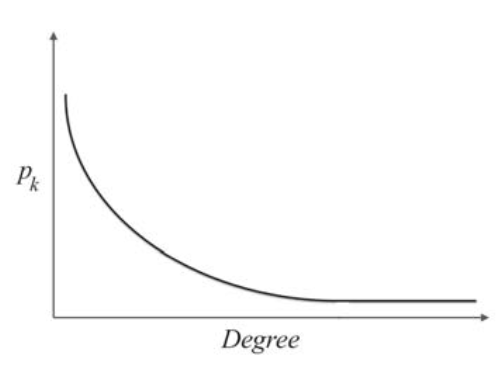
\includegraphics[scale=0.4]{power-law.png}
			
		\end{minipage}%
			
		
	\end{frame}
	
	%------------------------------------------------
	%  Propiedades de las redes: Coeficiente de agrupamiento por nodo
	\begin{frame}
		
		\frametitle{Propiedades de las redes: Coeficiente de agrupamiento por nodo}
		
		\begin{alertblock}{}
			Medida que describe el nivel en que los nodos de una red están agrupados entre sí.
		\end{alertblock}
		% Tendencia de los nodos a formar grupos densamente conectados.
		% Agrupamiento locales.
		
		\vspace{1\baselineskip}
		Por ejemplo:
		\begin{itemize}
			\item Red social: El coeficiente describe la probabilidad de la existencia de amistades que forman tríadas.
		\end{itemize}
		
		\vspace{1\baselineskip}
		Se calcula como:
		$$c_i = \frac{2E_i}{k_i(k_i - 1)}$$
	
		donde:
		\begin{itemize}
			\item $c_i$: coeficiente de agrupamiento para el nodo $i$
			\item $E_i$: cantidad de aristas que conectan los vecinos del nodo $i$
			\item $k_i$: cantidad de vecinos del nodo $i$
		\end{itemize}
		
	\end{frame}
	
	%------------------------------------------------
	%  Propiedades de las redes: Longitud del camino promedio
	\begin{frame}
		
		\frametitle{Propiedades de las redes: Longitud promedio del camino}
		
		\begin{itemize}
			
			\item Dos nodos cualesquiera están conectados a través de caminos cortos, siendo pequeña la longitud media del camino. \\[3mm]
			
			\item Esta propiedad es conocida como el fenómeno del mundo pequeño. \\[3mm] 
			
			\item Ejemplo: Conjetura de los 6 grados de separación
			\begin{alertblock}{}
				En una red de relaciones personales es posible conectar a cualquier par de personas a través de una trayectoria de como máximo seis individuos, siendo los seis grados de separación.
			\end{alertblock}
			
		\end{itemize}
		
	\end{frame}
	
	%------------------------------------------------
	%  Tipos de grafos según su topología
	\begin{frame}
		
		\frametitle{Tipos de grafos según la topología}
		
		Entender la topología de una red es una tarea imprescindible para el análisis y la extracción de información.
		
		\only<1>{
			\vspace{2\baselineskip}
			\textcolor{purple}{¿Qué tipos de red conocen a partir de su topología?}
		}
		
	\end{frame}
	
	%------------------------------------------------
	%  Tipos de grafos según su topología
	\begin{frame}
		
		\frametitle{Tipos de grafos según la topología}
		
		Entender la topología de una red es una tarea imprescindible. \\[4mm]
		
		\begin{itemize}
			
			\begin{minipage}{0.45\textwidth}
				
				\only<1-2>{
					\item Árbol y bosque
					
					\centering
					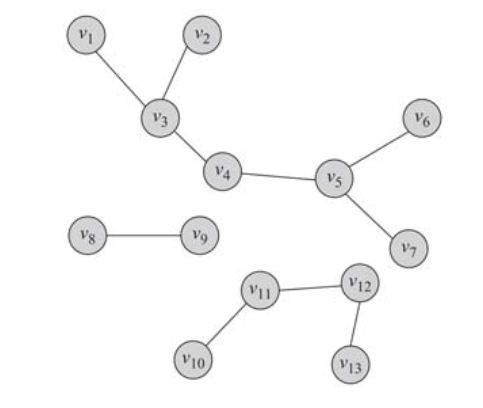
\includegraphics[scale=0.4]{arbol-bosque.png}
				}
				
				\only<3-4>{
					\item Grafo bipartito
					
					\centering
					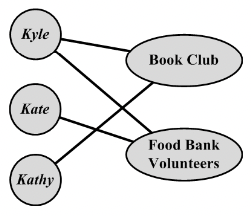
\includegraphics[scale=0.5]{grafo-bipartito.png}
				}
				
				\only<5>{
					\item Grafo regular
					
					\centering
					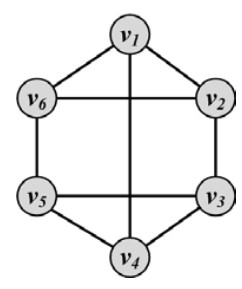
\includegraphics[scale=0.5]{grafo-regular.png}
				}
				
			\end{minipage}%
			\hfill
			\begin{minipage}{0.45\textwidth}
				
				\only<2-3>{
					\item Grafo completo
					
					\centering
					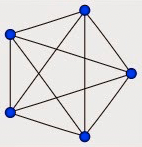
\includegraphics[scale=0.7]{grafo-completo.png}
				}
				
				\only<4-5>{
					\item Grafo planar
					
					\centering
					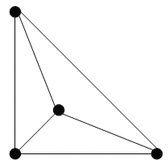
\includegraphics[scale=0.7]{grafo-planar.png}
				}
				
			\end{minipage}%
			
		\end{itemize}
		
	\end{frame}
	
	%------------------------------------------------
	%  Otros modelos de grafos
	\begin{frame}
		
		\frametitle{Otros modelos de grafos}
		
		Las problemáticas de la realidad han provocado el estudio de otros modelos de grafos, siendo estos:
		\begin{itemize}
			\item Modelo aleatorio
			\item Modelo de mundo pequeño
		\end{itemize}
		
		\vspace{2\baselineskip}
		
		Consideración:
		\begin{itemize}
			\item La existencia de una arista entre dos nodos es formada aleatoriamente.
		\end{itemize}
		
		\vspace{2\baselineskip}
		
	\end{frame}
	
	%------------------------------------------------
	%  Grafo aleatorio
	\begin{frame}
		
		\frametitle{Modelo aleatorio}
		
		\begin{alertblock}{}
			Un grafo $G$ es aleatorio si tiene $n$ nodos y la existencia de las aristas se define a partir de la probabilidad $p$. Se denota como $G(n, p)$.
		\end{alertblock}
		
		\vspace{1\baselineskip}
		
		El número esperado ($c$) de aristas conectadas a un nodo, o sea el grado esperado, es $(n-1)p$.
			
		\pause
		\vspace{2\baselineskip}
		
		Ejemplo de la evolución según los parámetros de creación
		
		\begin{minipage}{0.3\textwidth}
			
			Donde:
			\begin{itemize}
				\item $ds$: tamaño del diámetro 
				\item $slc$: mayor tamaño de la componente conexa
				\item $l$: longitud promedio del camino
			\end{itemize}
			
		\end{minipage}%
		\hfill
		\begin{minipage}{0.6\textwidth}
			
			%\centering
			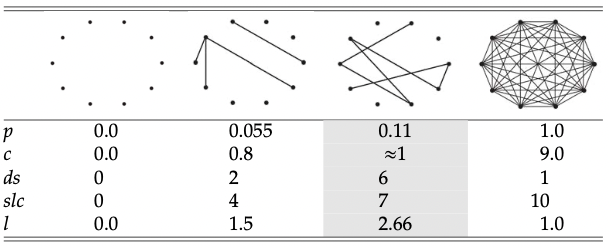
\includegraphics[scale=0.4]{evolucion-grafo-aleatorio.png}
			
			% Cuando p es pequeña:
			%	- no hay grandes componentes y las formadas son aisladas.
			%	- los valores  del diámetro son pequeños.
			
			% Caundo p aumenta:
			%	- comienza aparecer componentes grandes.
			%	- las componentes aisladas se conectan.
			%	- llos valores del diámetro aumentan.
		
		\end{minipage}%
		
		% Deficiencias:
		% 	- subestima el coeficiente de agrupación.
		% 	- Vulnerabilidad a fallos aleatorios: Los grafos aleatorios son relativamente resistentes a fallos aleatorios, ya que la eliminación de nodos individuales tiende a tener un impacto limitado en la conectividad general de la red. Esto se debe a la falta de estructura organizada en el grafo.
		% 	- Ausencia de estructura de comunidad: En un grafo aleatorio, no hay una estructura de comunidad clara o grupos densamente conectados de nodos. La formación de comunidades en un grafo aleatorio es puramente el resultado de la probabilidad aleatoria de conexión entre nodos.
		
	\end{frame}
	
	%------------------------------------------------
	%  Grafo de mundo pequeño
	\begin{frame}
		
		\frametitle{Modelo de mundo pequeño}
		
		\begin{itemize}
			\item La topología es similar a un anillo porque se forma a partir de un anillo regular entramado. \\[2mm]
		\end{itemize}
			
			\begin{minipage}{0.45\textwidth}
				
				\begin{alertblock}{}
					Un grafo de anillo regular entramado (\emph{regular ring lattice}) es un caso especial de los grafos regulares, donde existe cierto patrón de cómo los nodos ordenados se conectan entre sí, es decir, 
					$$\forall v_i, v_j \in V, \exists <x_i, x_j> \in E \Leftrightarrow 0 < |i - j| < \frac{c}{2}$$ 
					donde $V$ el conjunto de nodos, $E$ el conjunto de las aristas del grafo y $c$ es el grado de cada nodo.
				\end{alertblock}
				
			\end{minipage}%
			\hfill
			\begin{minipage}{0.45\textwidth}
				
				\centering
				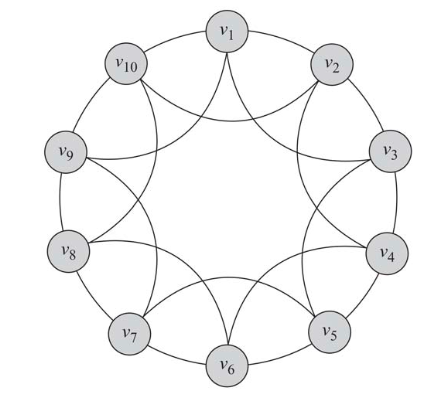
\includegraphics[scale=0.35]{anillo-regular.png}
				
				Anillo regular de grado $4$
			\end{minipage}%
			
	\end{frame}
	
	%------------------------------------------------
	%  Algoritmo para crear un grafo de mundo pequeño
	%  \begin{frame}
	%  
	%  	\frametitle{Algoritmo para crear un grafo de mundo pequeño}
	%  	
	%  	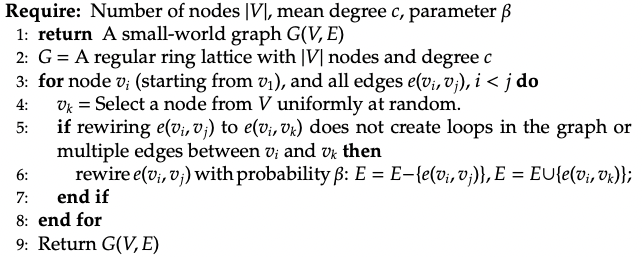
\includegraphics[scale=0.6]{algoritmo-mundo-pequenno.png}
		
	%  	\vspace{2\baselineskip}
	%  	$\beta$ probabilidad de sustituir una arista 
	%  \end{frame}
	
	%------------------------------------------------
	%  Ejemplo de la creación de un grafo mundo pequeño
	\begin{frame}
		
		\frametitle{Ejemplo de la creación de un grafo mundo pequeño}
		
		\centering
		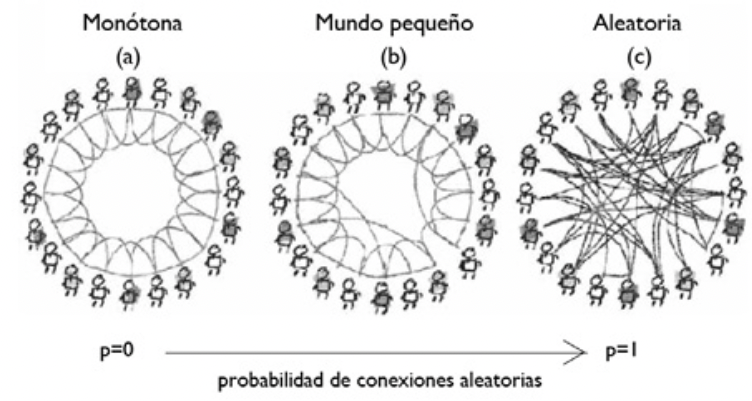
\includegraphics[scale=0.4]{mundo-pequenno.png}
		% Aquí p es la probabilidad de selecciponar una arista y reconectarla con otro par de nodos.
		
		{\scriptsize Tomado de 	\url{https://www.revistas.una.ac.cr/index.php/ensayospedagogicos/article/view/9338/11078}}
	
	\end{frame}
	
	%------------------------------------------------
	%  Propiedades de los grafos de mundo pequeño
	\begin{frame}
		
		\frametitle{Propiedades de los grafos de mundo pequeño}
		
		\begin{itemize}
			
			\item Cortas distancias promedio \\[2mm]
			% A pesar de tener un gran número de nodos, la distancia promedio entre pares de nodos es relativamente corta. Esto significa que, en promedio, los nodos están relativamente cerca unos de otros en términos de la cantidad de enlaces que deben seguir para conectarse.
			
			\item Alto coeficiente de agrupamiento \\[2mm]
			% A pesar de las distancias cortas promedio, los nodos tienden a formar agrupaciones densamente conectadas o "clústeres". Esto se refleja en un coeficiente de agrupamiento global significativamente mayor que el esperado en un grafo aleatorio.
			
			\item Presencia de ``puentes'' o ``conectores'' \\[2mm]
			% Aunque la red está altamente agrupada, también contiene algunos nodos que actúan como "puentes" entre diferentes grupos o clústeres. Estos nodos conectores facilitan la transmisión eficiente de información o influencia a través de la red.
			
			\item Resistencia a fallos aleatorios pero vulnerabilidad a ataques dirigidos \\[2mm]
			% Los grafos de mundo pequeño tienden a ser resistentes a la eliminación aleatoria de nodos debido a la presencia de múltiples rutas entre pares de nodos. Sin embargo, son vulnerables a ataques dirigidos contra los nodos altamente conectados (hubs), ya que la eliminación de estos nodos puede fragmentar la red en múltiples componentes.
		\end{itemize}
	
	\end{frame}
	
	%------------------------------------------------
	% Break
	{
		\setbeamertemplate{background canvas}
		{%
			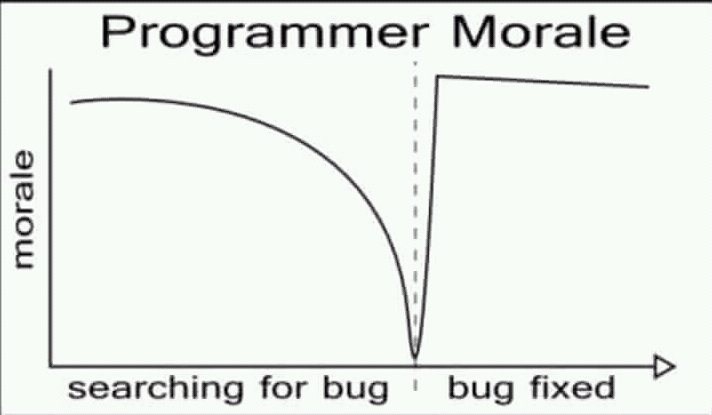
\includegraphics[width=\paperwidth,height=\paperheight]{break1.png}
		}
		
		\begin{frame}
		\end{frame}
	}
	
	%------------------------------------------------
	%  
	\begin{frame}
		
		\frametitle{Obtener información de una red según la topología}
		
		\begin{itemize}
			\item PageRank \\[2mm]
			% Analiza la importancia relativa de los nodos 
			
			\item Hypertext Induced Topic Selection (HITS) \\[2mm]
			% Analiza la importancia relativa de los nodos , pero se basa en la nociión de nodos "autoridad" y "hub"
			
			\item Índices de centralidad \\[2mm]
			% Medida numérica que indica la importancia o el grado de centralidad de un nodo en una red
			
			\item Detección de comunidades
			% Se refieren a conjuntos de nodos altamente interconectados entre sí y relativamente menos conectados con nodos fuera del conjunto. Identificar comunidades en un grafo es un aspecto importante del análisis de redes, ya que proporciona información sobre la estructura modular y la organización de la red.
			
		\end{itemize}
		
	\end{frame}
	
	%------------------------------------------------
	%  Centralidad de un nodo
	\begin{frame}
		
		\frametitle{Centralidad de un nodo}
		
		\begin{alertblock}{}
			Término general para referirse a cualquier medida numérica que indique la importancia o el grado de centralidad de un nodo en una red. 
		\end{alertblock}
		
		\vspace{2\baselineskip}
		
		Medidas para computar la centralidad de un nodo:
		\begin{itemize}
			\item Centralidad de grado
			\item Centralidad de cercanía
			\item Centralidad de intermediación
			\item Centralidad de vector propio
		\end{itemize}
		
	\end{frame}
	
	%------------------------------------------------
	%  Centralidad de grado
	\begin{frame}
		
		\frametitle{Centralidad de grado}
		
		\begin{minipage}{0.45\textwidth}
			
			\begin{itemize}
				\item Mide la importancia de un nodo según su número de aristas.
			\end{itemize}
			
		\end{minipage}%
		\hfill
		\begin{minipage}{0.45\textwidth}
			
			\centering
			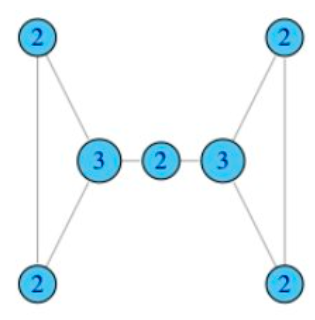
\includegraphics[scale=0.4]{centralidad-grado.png}
			
		\end{minipage}%
		
	\end{frame}
	
	%------------------------------------------------
	%  Centralidad de cercanía
	\begin{frame}
		
		\frametitle{Centralidad de cercanía (\emph{Closeness})}
		
		\begin{minipage}{0.45\textwidth}
			
			\begin{itemize}
				\item Mide la importancia de un nodo según su distancia promedio a todos los demás nodos en la red. 
				
				\item Se calcula como:
				$$C_c(v_i) = \frac{1}{\frac{1}{n-1} \sum_{v_j \neq v_i} l_{i,j}}$$
				
				donde:
				\begin{itemize}
					\item $v_i, v_j \in V$
					\item $n = |V|$
					\item $l_{i, j}$: menor distancia del camino del nodo $v_i$ a $v_j$
				\end{itemize}
				
				% \item Los nodos que están más cerca de todos los demás nodos tienen un mayor valor de centralidad.
			\end{itemize}
			
		\end{minipage}%
		\hfill
		\begin{minipage}{0.45\textwidth}
			
			\centering
			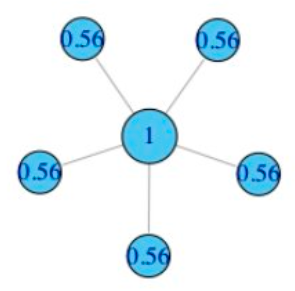
\includegraphics[scale=0.4]{centralidad-cercania.png}
			
		\end{minipage}%
		
	\end{frame}
	
	%------------------------------------------------
	%  Centralidad de intermediación
	\begin{frame}
		
		\frametitle{Centralidad de intermediación (\emph{Betweenness})}
		
		\begin{minipage}{0.45\textwidth}
			
			\begin{itemize}
				\item Mide la importancia de un nodo según la cantidad de veces que aparece en los caminos más cortos entre todos los pares de nodos en la red.
				
				\item Se calcula como:
				$$C_b(v_i) = \sum_{s \neq t \neq v_i} \frac{\sigma_{st}(v_i)}{\sigma_{st}}$$
				
				donde:
				\begin{itemize}
					\item $v_i, s, t \in V$
					\item $\sigma_{st}$: cantidad de caminos cortos entre los nodos $s$ y $t$ 
					\item $\sigma_{st}(v_i)$: cantidad de caminos cortos entre los nodos $s$ y $t$ que pasan por $v_i$
				\end{itemize}
				
				\item Se normaliza por el máximo valor obtenido.
			\end{itemize}
			
		\end{minipage}%
		\hfill
		\begin{minipage}{0.45\textwidth}
			
			\centering
			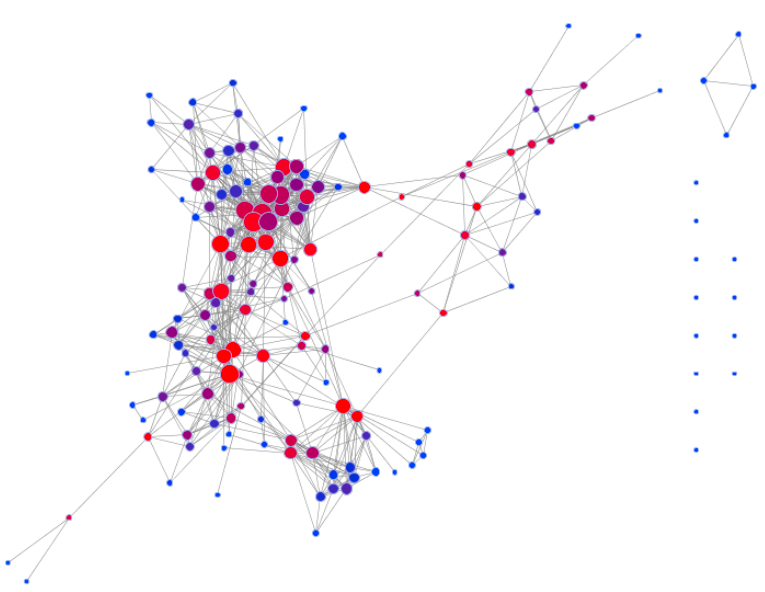
\includegraphics[scale=0.35]{centralidad-intermediacion.png}
			
		\end{minipage}%
		
	\end{frame}
	
	%------------------------------------------------
	%  Centralidad de vector propio
	\begin{frame}
		
		\frametitle{Centralidad de vector propio}
		
		\begin{minipage}{0.45\textwidth}
			
			\begin{itemize}
				\item Mide la importancia de un nodo según la importancia de sus vecinos.
				
				\item Se calcula como:
				$$C_e(v_i) = \frac{1}{\lambda} \sum_{j = 1}^{n} A_{j, i}C_e(v_j)$$
				
				donde:
				\begin{itemize}
					\item $v_i \in V$
					\item $n = |V|$
					\item $A$: matriz de adyacencia
					\item $\lambda$: valor propio (constante)
				\end{itemize}
				
				\item Cálculo iterativo.
			\end{itemize}
			
		\end{minipage}%
		\hfill
		\begin{minipage}{0.45\textwidth}
			
			\centering
			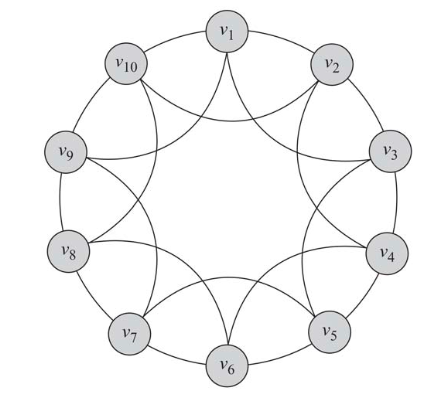
\includegraphics[scale=0.35]{anillo-regular.png}
			
		\end{minipage}%
		
	\end{frame}
	
	%------------------------------------------------
	%  Diferencias entre las medidas de centralidad
	\begin{frame}
		
		\frametitle{Diferencias entre las medidas de centralidad}
		
		\centering
		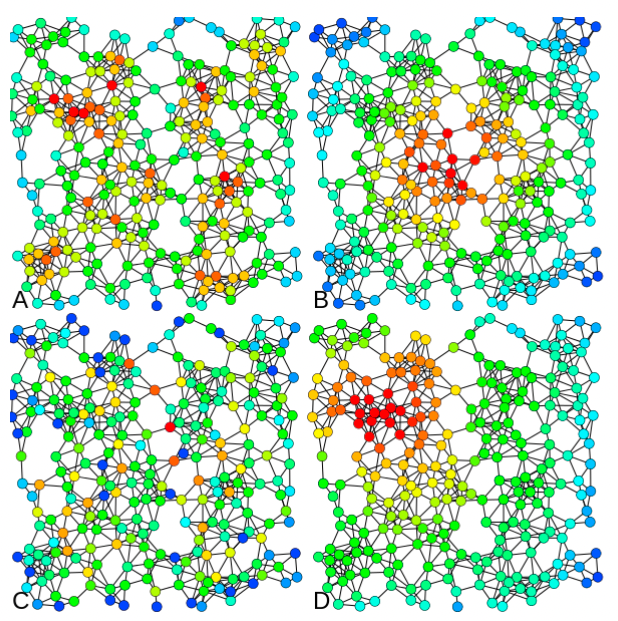
\includegraphics[scale=0.3]{ejemplo-centralidad.png}
		
		
\includegraphics[scale=0.27]{ejemplo-centralidad-etiquetas.png}
		
	\end{frame}
	
	%------------------------------------------------
	%  Detección de comunidades
	\begin{frame}
		
		\frametitle{Detección de comunidades}
		
		No existe un consenso sobre lo que es una \textbf{comunidad} dentro de una red. Aunque pudiese definirse como:
		
		% \vspace{1\baselineskip}
		
		\begin{alertblock}{Comunidad}
			En el contexto de las redes, se refiere a un conjunto de nodos que están más densamente interconectados entre sí que con los nodos fuera del conjunto.
		\end{alertblock}
		
		\only<2>{
			\vspace{3\baselineskip}
				\textcolor{purple}{¿Qué ideas pueden usarse para detectar comunidades dentro de una red?} 
		}
		
	\end{frame}
	
	%------------------------------------------------
	%  Ideas para detectar comunidades dentro de una red
	\begin{frame}
		
		\frametitle{Ideas para detectar comunidades dentro de una red}
		
		\begin{minipage}{0.35\textwidth}
			
			\begin{itemize}
				\item Mutualidad de los enlaces \\[2mm]
				% Todos los nodos están interconctados 
				
				\item Frecuencia de enlaces \\[2mm]
				% Cada nodos tienen k enlaces con el resto
				
				\item Alcance entre los nodos 
				% Los nodos se separan por a lo sumo n saltos
				
			\end{itemize}
		
		\end{minipage}%
		\hfill
		\begin{minipage}{0.6\textwidth}
		
			\pause
			\centering
			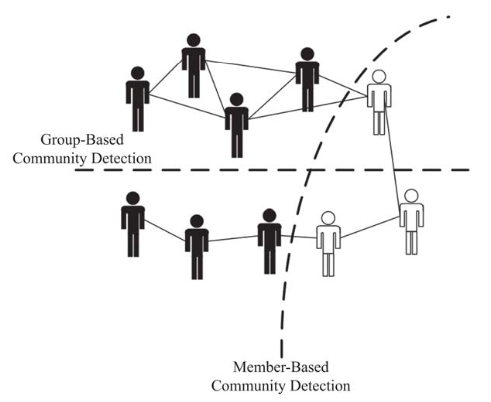
\includegraphics[scale=0.45]{tipos-de-comunidades.png}
		
		\end{minipage}%
		
		
	\end{frame}
	
	%------------------------------------------------
	%  Algoritmos para detectar comunidades
	\begin{frame}
		
		\frametitle{Algoritmos para detectar comunidades basados en los miembros}
		
		\begin{minipage}{0.55\textwidth}
			
			\begin{itemize}
				\item Idea: Buscar conjuntos donde los nodos tengan características similares. \\[0.5mm]
				
				\item Se enfoca en localizar cliques.
			
				\begin{alertblock}{Clique}
					Sea el grafo $G(V, E)$, $C$ es un clique de G si $\forall x_i, x_j \in V(C) \Rightarrow <x_i, x_j> \in E(C)$. 
				\end{alertblock} 
				
				\vspace{0.5\baselineskip}
				
				\item Problemas a enfrentar:
				\begin{itemize}
					\item Solapamiento
					\item Complejidad computacional \\[0.5mm]
				\end{itemize}
				
				\item Se intenta ``relajar'' el concepto de clique, buscando conjuntos de no maximales y/o conjunto con un diámetro predefinido.
				
			\end{itemize}
			
		\end{minipage}%
		\hfill
		\begin{minipage}{0.35\textwidth}
			
			\centering
			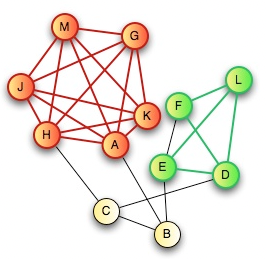
\includegraphics[scale=0.6]{clique.png}
			
		\end{minipage}%
		
	\end{frame}
	
	%------------------------------------------------
	%  Algoritmos para detectar comunidades basados en el grupo
	\begin{frame}
		
		\frametitle{Algoritmos para detectar comunidades basados en el grupo}
		
		\begin{itemize}
			\item Idea: Encontrar grupos de nodos donde cada grupo presenta ciertas características. \\[2mm]
			
			\item Ejemplos de métodos usados:
			\begin{itemize}
				\item Agrupamiento jerárquico
				\item K-Means
				\item Particionamiento a través de funciones de costo \\[2mm]
			\end{itemize}
		
			\item Problemas a enfrentar:
			\begin{itemize}
				\item La eliminación de una arista repercute en el análisis global
				\item Depende de condiciones iniciales \\[2mm]
			\end{itemize}
			
		\end{itemize}
			
	\end{frame}
	
	%------------------------------------------------
	% Break
	\begin{frame}
		
		\centering
		
\includegraphics[height=\paperheight]{fin.png}
		
	\end{frame}

	
	%------------------------------------------------
	% Conclusiones
	\begin{frame}
		
		\frametitle{Conclusiones}
		
		\begin{itemize}
			
			\item La estructura de una red es fundamental para comprender su funcionamiento y dinámica. Los conceptos de topología, propiedades y modelos de redes proporcionan una base sólida para analizar y entender diferentes tipos de redes en una variedad de campos. \\[4mm]
			
			\item La detección de comunidades y la centralidad del nodo son herramientas poderosas para identificar patrones y estructuras importantes en las redes. Estas medidas proporcionan información valiosa sobre la organización y la importancia de los nodos en una red, así como sobre la dinámica de la interacción entre ellos.
			
		\end{itemize}
		
	\end{frame}

	%------------------------------------------------
	% Bibliografía
	\begin{frame}
		
		\frametitle{Bibliografía}
		
		\begin{itemize}
						
			\item Zafarani, Reza; Abbasi, Mohammad Ali; Liu, Huan. ``Social Media Mining. An Introduction''. 2014. Cambridge University Press. Capítulos I, II.
			     
		\end{itemize}
		
	\end{frame}
	
	%------------------------------------------------
	% Fin
	\begin{frame}
		\titlepage
	\end{frame}
	
	
	
\end{document} 